\section{Signal Phase Difference}
\label{sec:02_phase}

With a different approach to the correlation methods, the \ac{TDOA} can be
detected by observing the phase of one reference frequency $f_c$.
Imaging a single-sinusoidal signal moving from left to right as
pictured in \cref{fig:02_phaseTheory}, two distant sensors
(\textit{channel 2} and \textit{channel 3}) will
receive different parts of the signal at the same time.
Transforming the frames into frequency domain by \ac{FFT}, the pase of the
maximal frequency differ by the delay.
% -------------------------------------------------------------

\begin{figure}[ht]
	\centering
		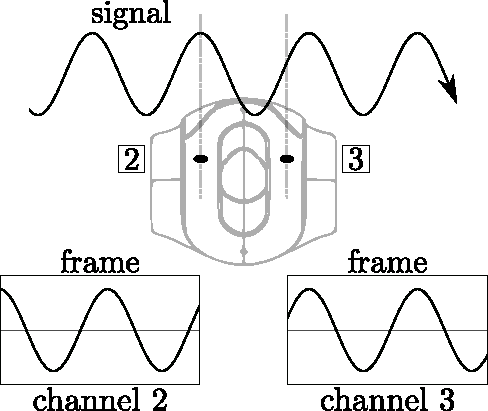
\includegraphics[width=0.35\columnwidth]{figures/phase_theory}
	\caption{Explanatory illustration of the phase difference method.}
    \label{fig:02_phaseTheory}
\end{figure}
% -------------------------------------------------------------

The phase of a signal's reference frequency is easily computable in frequency domain
with
\bal
    \phi(f_c) &= tan^{-1}\left(\frac{imag(X(f_c))}{real(X(f_c))}\right).
\eal
% -------------------------------------------------------------
With the difference of the phases of two channel, the delay in meters is defined as
\bal
    D &= \frac{\Delta \phi \cdot c_s}{2 \pi \cdot f_c}.
\eal
From that, the direction angle calculation of \cref{eq:02_tdoaAngle} can
be followed.
It should be noted that certain requirements needs to be fulfilled to receive a
unambiguous result due to signal periodicity.
\Cref{subsubsec:03_phase} covers the conditions that apply for this thesis's
hardware.
% -------------------------------------------------------------